\section{Random Networks}
In network theory, random networks play a crucial role in understanding the structure and behavior of complex systems. These networks are often used to model real-world networks, such as the Internet and social networks. There are several methods to generate random networks, each with its own specific focus, such as the degree distribution, the average path length, or the presence of particular structural properties. In this section, we will explore some of the most important models used to generate random networks, highlighting their characteristics and differences.

\subsection{Erd\H{o}s-Rényi Random Graph}

The Erd\H{o}s-Rényi (E-R) random graph $G(N,M)$, where $N$ and $M$ are the number of nodes and links respectively, is one of the first attempts to generate a random network \cite{erdos-renyi1960}. The network is built by randomly choosing $M$ links from all the possible ones. Usually, is used the variation proposed by Gilbert $G(N,p)$ \cite{gilbert} , where $p$ is the probability that two distinct node are connected. The two formulations converge in the thermodynamic limit $N \rightarrow \infty$ and they are interchangeable.
This type of random graph has peculiar properties, such as the degree distribution of the nodes $P(k)$ is binomial
\begin{equation}
    P(k) = \binom{n-1}{k}p^k(1-p)^{n-1-k}
\end{equation} 
Additionally, if $p > \frac{1}{N}$ then is almost sure that the network presents a giant component.
In this work we use the second approach. Figure \ref{E-R_example} shows two examples of E-R random graph, one below and one above the giant component threshold.

\begin{figure}[ht!]
    \centering
    \begin{subfigure}[t]{0.49\textwidth}
        \centering
        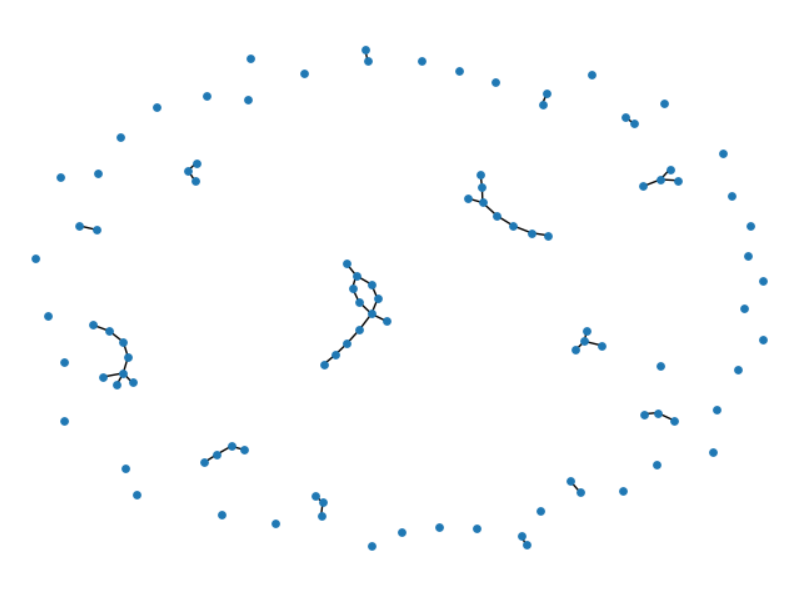
\includegraphics[width=\linewidth]{image/E_R_N100_p0,01.png}
    \end{subfigure}
    \hfill
    \begin{subfigure}[t]{0.49\textwidth}
        \centering
        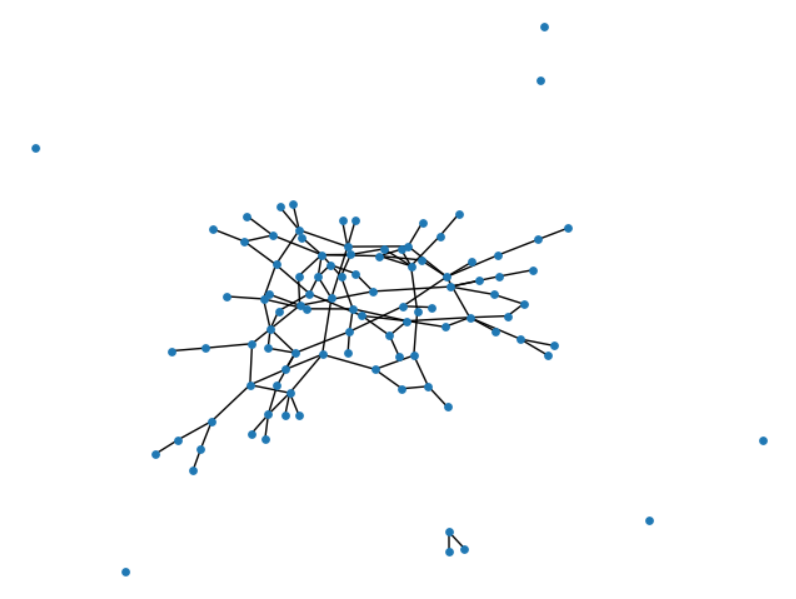
\includegraphics[width=\linewidth]{image/E_R_N100_p0,02.png}
    \end{subfigure}
    \caption{Two examples of Erd\H{o}s-Rényi random graphs: on the left, it has 100 nodes and $p = 0.01$; on the right, it has 100 nodes and $p = 0.02$. Overcoming the threshold $p > 0.01$ can be seen the formation of the giant component.}
    \label{E-R_example}
\end{figure}
%the algorithm is define as below :
%\begin{enumerate}
 %   \item we identify the graph by its adjacency matrix;
 %   \item For each possible link, we generate a random number, if it is less than $p$ the respective entry in the adjacency matrix  is 1 otherwise 0.
%\end{enumerate}

However, the E-R algorithm does not produce networks similar to those found in nature which tend to be more clustered and to have hubs (nodes with very high degree). To simulate these properties, new algorithms have been proposed like the Barab\'abi-Albert scale-free network and the Watts-Strogatz small-world network.

\subsection{Barab\'abi-Albert Scale-Free Network}
Barab\'abi and Albert (B-A) proposed a scale-free network $G(N, m)$, where $N$ is the number of nodes and $m$ is a parameter, that mimics the behavior of real graph like the Internet \cite{Barabasi_Albert_1999}. This type of graph exhibits some preferential nodes which have a degree order of magnitude higher than the average and it presents a power law as degree distribution.
The model works by preferential attachment, where new nodes are more likely to connect to nodes that already have a higher degree. 

The algorithm is defined as follow:
\begin{enumerate}
    \item It is initialized a complete graph of $m_0 > m$ node, usually $m_0 = m+1$;
    \item The other nodes are connected to this graph: for each new node, it is connected to $m$ nodes with probability $p_i = \frac{k_i}{\sum_i k_i}$, where $k_i$ is the degree of the $i$ node.
\end{enumerate}
Figure \ref{B-A_example} shows two examples of B-A networks.

\begin{figure}[ht!]
    \centering
    \begin{subfigure}[t]{0.49\textwidth}
        \centering
        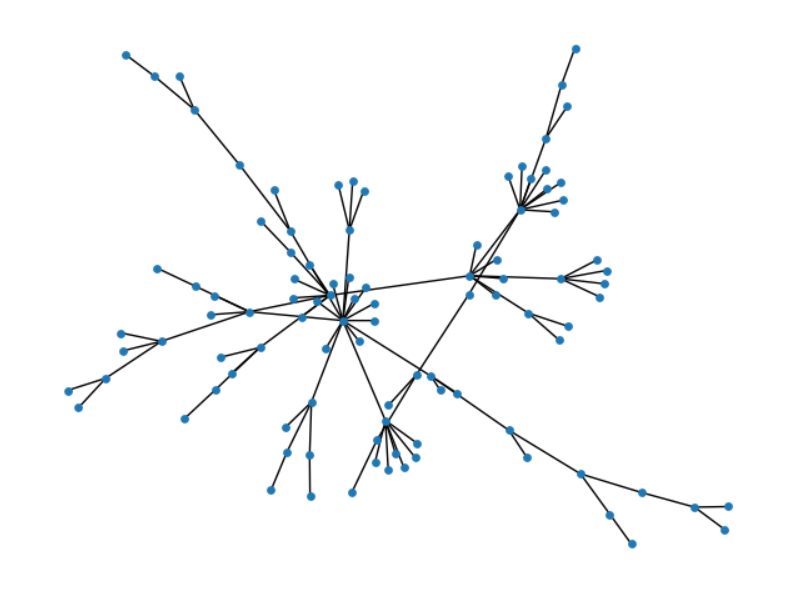
\includegraphics[width=\linewidth]{image/B_A_N100_m1.png}
    \end{subfigure}
    \hfill
    \begin{subfigure}[t]{0.49\textwidth}
        \centering
        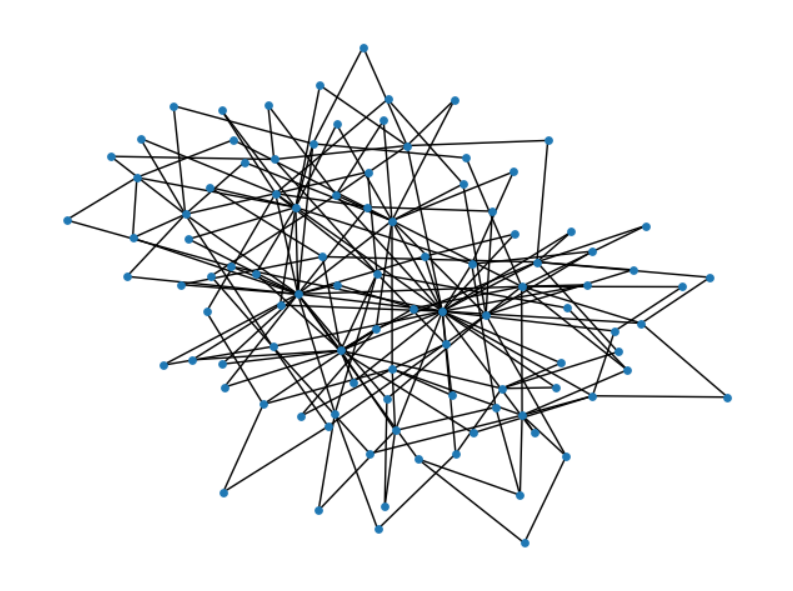
\includegraphics[width=\linewidth]{image/B_A_N100_m2.png}
    \end{subfigure}
    \caption{Two example of Barab\'abi-Albert scale-free networks: on the left, it has 100 nodes and $m=1$; on the right, it has 100 nodes and $m=2$.}
    \label{B-A_example}
\end{figure}

\subsection{Watts-Strogatz Small World Network}

The Watts-Strogatz small-world network $G(N, K, p)$, where $N$ is the number of nodes, $K$ is the average degree (it must be even) and $p$ is the rewiring probability, is a model that exhibits high clustering and short average path lengths \cite{Watts-Strogatz_1998}. The degree distribution follows a power law and the network is homogeneous, meaning that all nodes have similar degree.

The algorithm is defined as follows:
\begin{enumerate}
    \item A ring network with $N$ nodes is created, where each node is connected to the $K/2$ nearest neighbors on each side;
    \item For each edge, with probability $p$ the link is removed and a new one is created to random node. There is no preferential attachments. The new link must be a not existing one.
\end{enumerate}

Figure \ref{W-S_example} it shows two example of W-S networks.

\begin{figure}[ht!]
    \centering
    \begin{subfigure}[t]{0.49\textwidth}
        \centering
        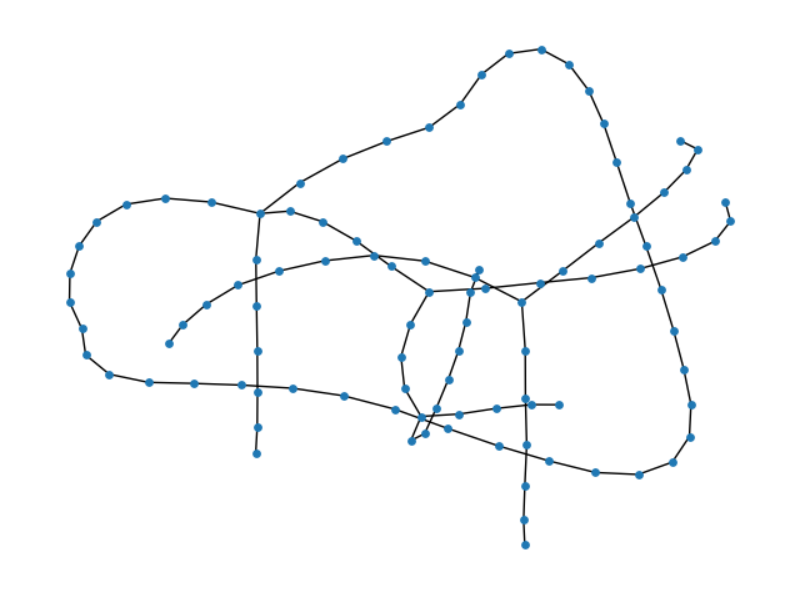
\includegraphics[width=\linewidth]{image/W_S_N100_K2_p0,1.png}
    \end{subfigure}
    \hfill
    \begin{subfigure}[t]{0.49\textwidth}
        \centering
        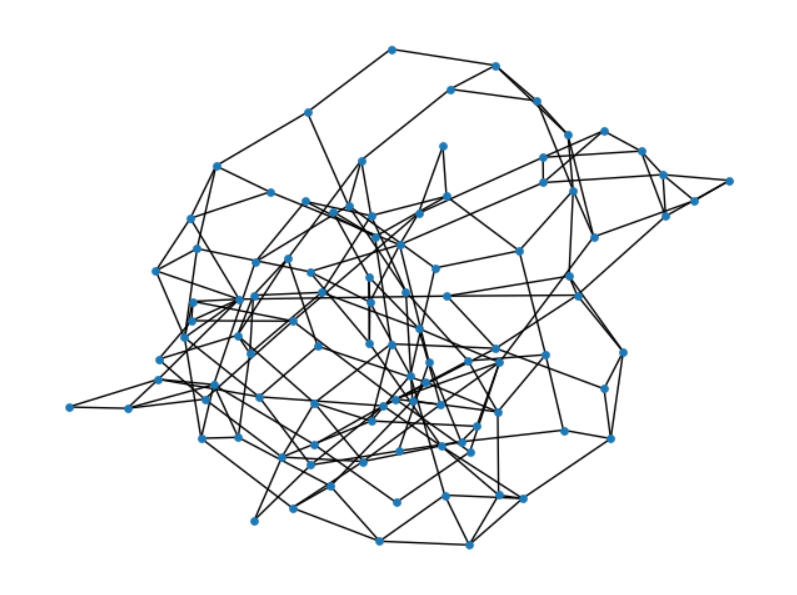
\includegraphics[width=\linewidth]{image/W_S_N100_K4_p0,3.png}
    \end{subfigure}
    \caption{Two example of Watts-Strogatz small world networks: on the left, it has 100 nodes, $K=2$ and $p=0.1$; on the right, it has 100 nodes, $K=4$ and $p=0.3$.}
    \label{W-S_example}
\end{figure}

The B-A and W-S algorithms produce more realistic networks compared to the E-R one, but both focus on their specific feature: the B-A networks fail to reproduce the high clustering of real networks and the W-S ones fail to reproduce the hubs characteristic of networks like Internet.